\section{Extracted evidence boundary}\label{app:evidence-boundary}
The numerical values reproduced in Sections~\ref{sec:rank-two-alignment},
\ref{sec:bounded-decisions}, \ref{sec:rank-three}, and~\ref{sec:wannier-bridge}
originate from the preserved
\texttt{docs/publications/papers/Ragasa2026a/v2/manuscript.tex} and its cited retained
calculations. This
appendix records their permitted role in the present study.

\begin{center}\small
\begin{tabularx}{\textwidth}{YYY}
\toprule
\textbf{Extracted component} & \textbf{Supported statement} & \textbf{Not supported} \\
\midrule
M3 constrained rank-two admissible sets & One frozen finite alignment family has an explicit nonidentity-aligned common witness and, at a tighter operator threshold, a certified positive separation & Continuous or momentum-dependent alignment, higher-rank validity, material validity, or transferable thresholds \\
M2 rank-two alignment control & A known pointwise inverse attack is recoverable while one global unitary leaves a finite residual, and the attack changes finite-range compressibility & General alignment optimizer, continuum decay law, or material validity \\
Rank-three smooth/rough frames & Finite-mesh equality of spectra and Wilson-phase multisets can coexist with different spread estimators and hopping tails & Continuum topology, material validity, or global localization optimum \\
Synthetic Wannier90 bridge & One algorithm-selected rank-three frame can be identified pointwise with the direct retained subspace while differing under a restricted global family & Mesh-independent MLWF convergence, global basin optimality, or first-principles validation \\
Procrustes construction & Pointwise and one-global unitary alignments solve different declared least-squares problems when their overlap factors are qualified & Permission to complete a rank-deficient map or enlarge the admissible family after observing results \\
\bottomrule
\end{tabularx}
\end{center}

A post-hoc exact reanalysis of the sealed M3 training quadratics places the compatibility
transition at $\tau_H=0.3192641695$ for the fixed $\tau_E=0.03$ and the declared
nine-angle family. It is sensitivity characterization, not a prospectively frozen
prediction or physical threshold calibration.

\begin{figure}[htbp]
\centering
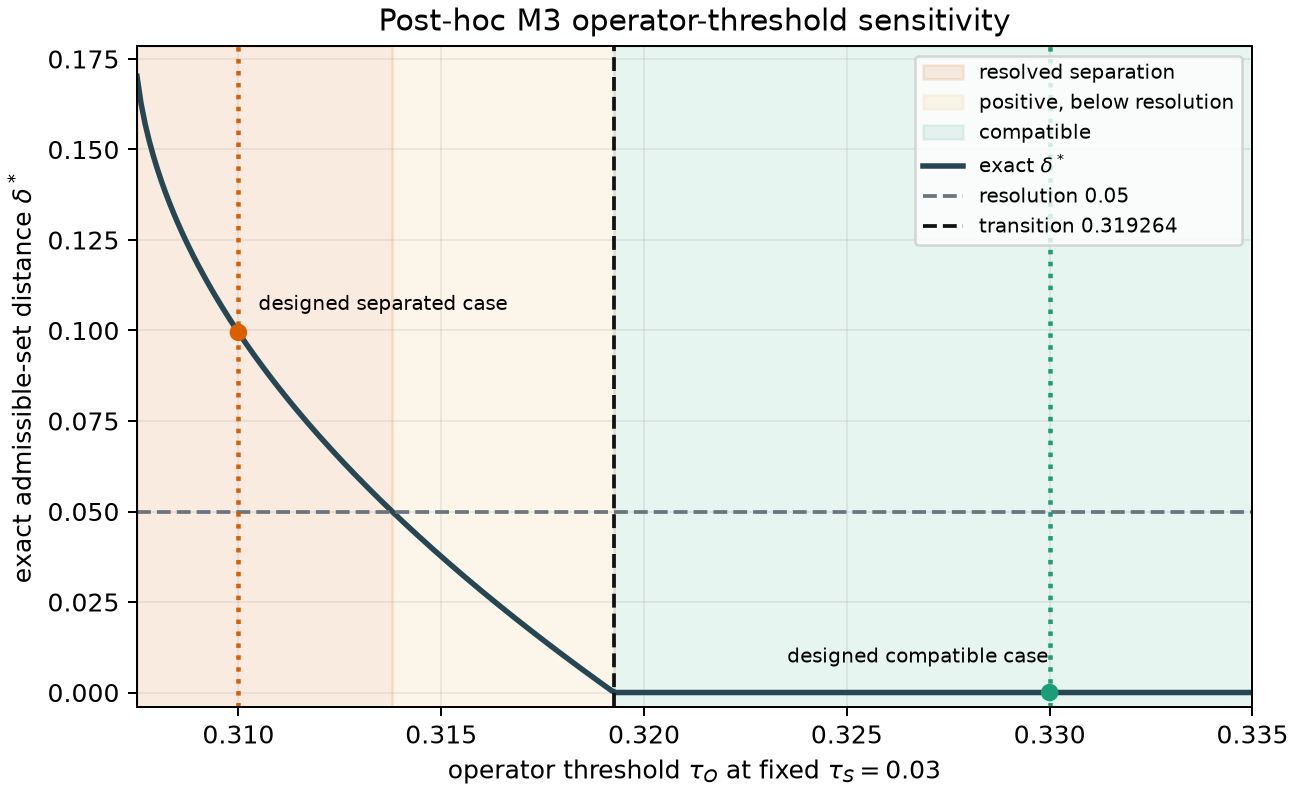
\includegraphics[width=0.84\textwidth]{../../../../../calculations/ICMSEP2026/conference/paper_1/constrained-admissible-sets-threshold-sensitivity/operator-threshold-sensitivity.png}
\caption{Post-hoc M3 operator-threshold sensitivity. The sealed compatible and separated
thresholds lie on opposite sides of the exact finite-family transition.}
\label{fig:m3-threshold-sensitivity}
\end{figure}

\begin{figure}[htbp]
\centering
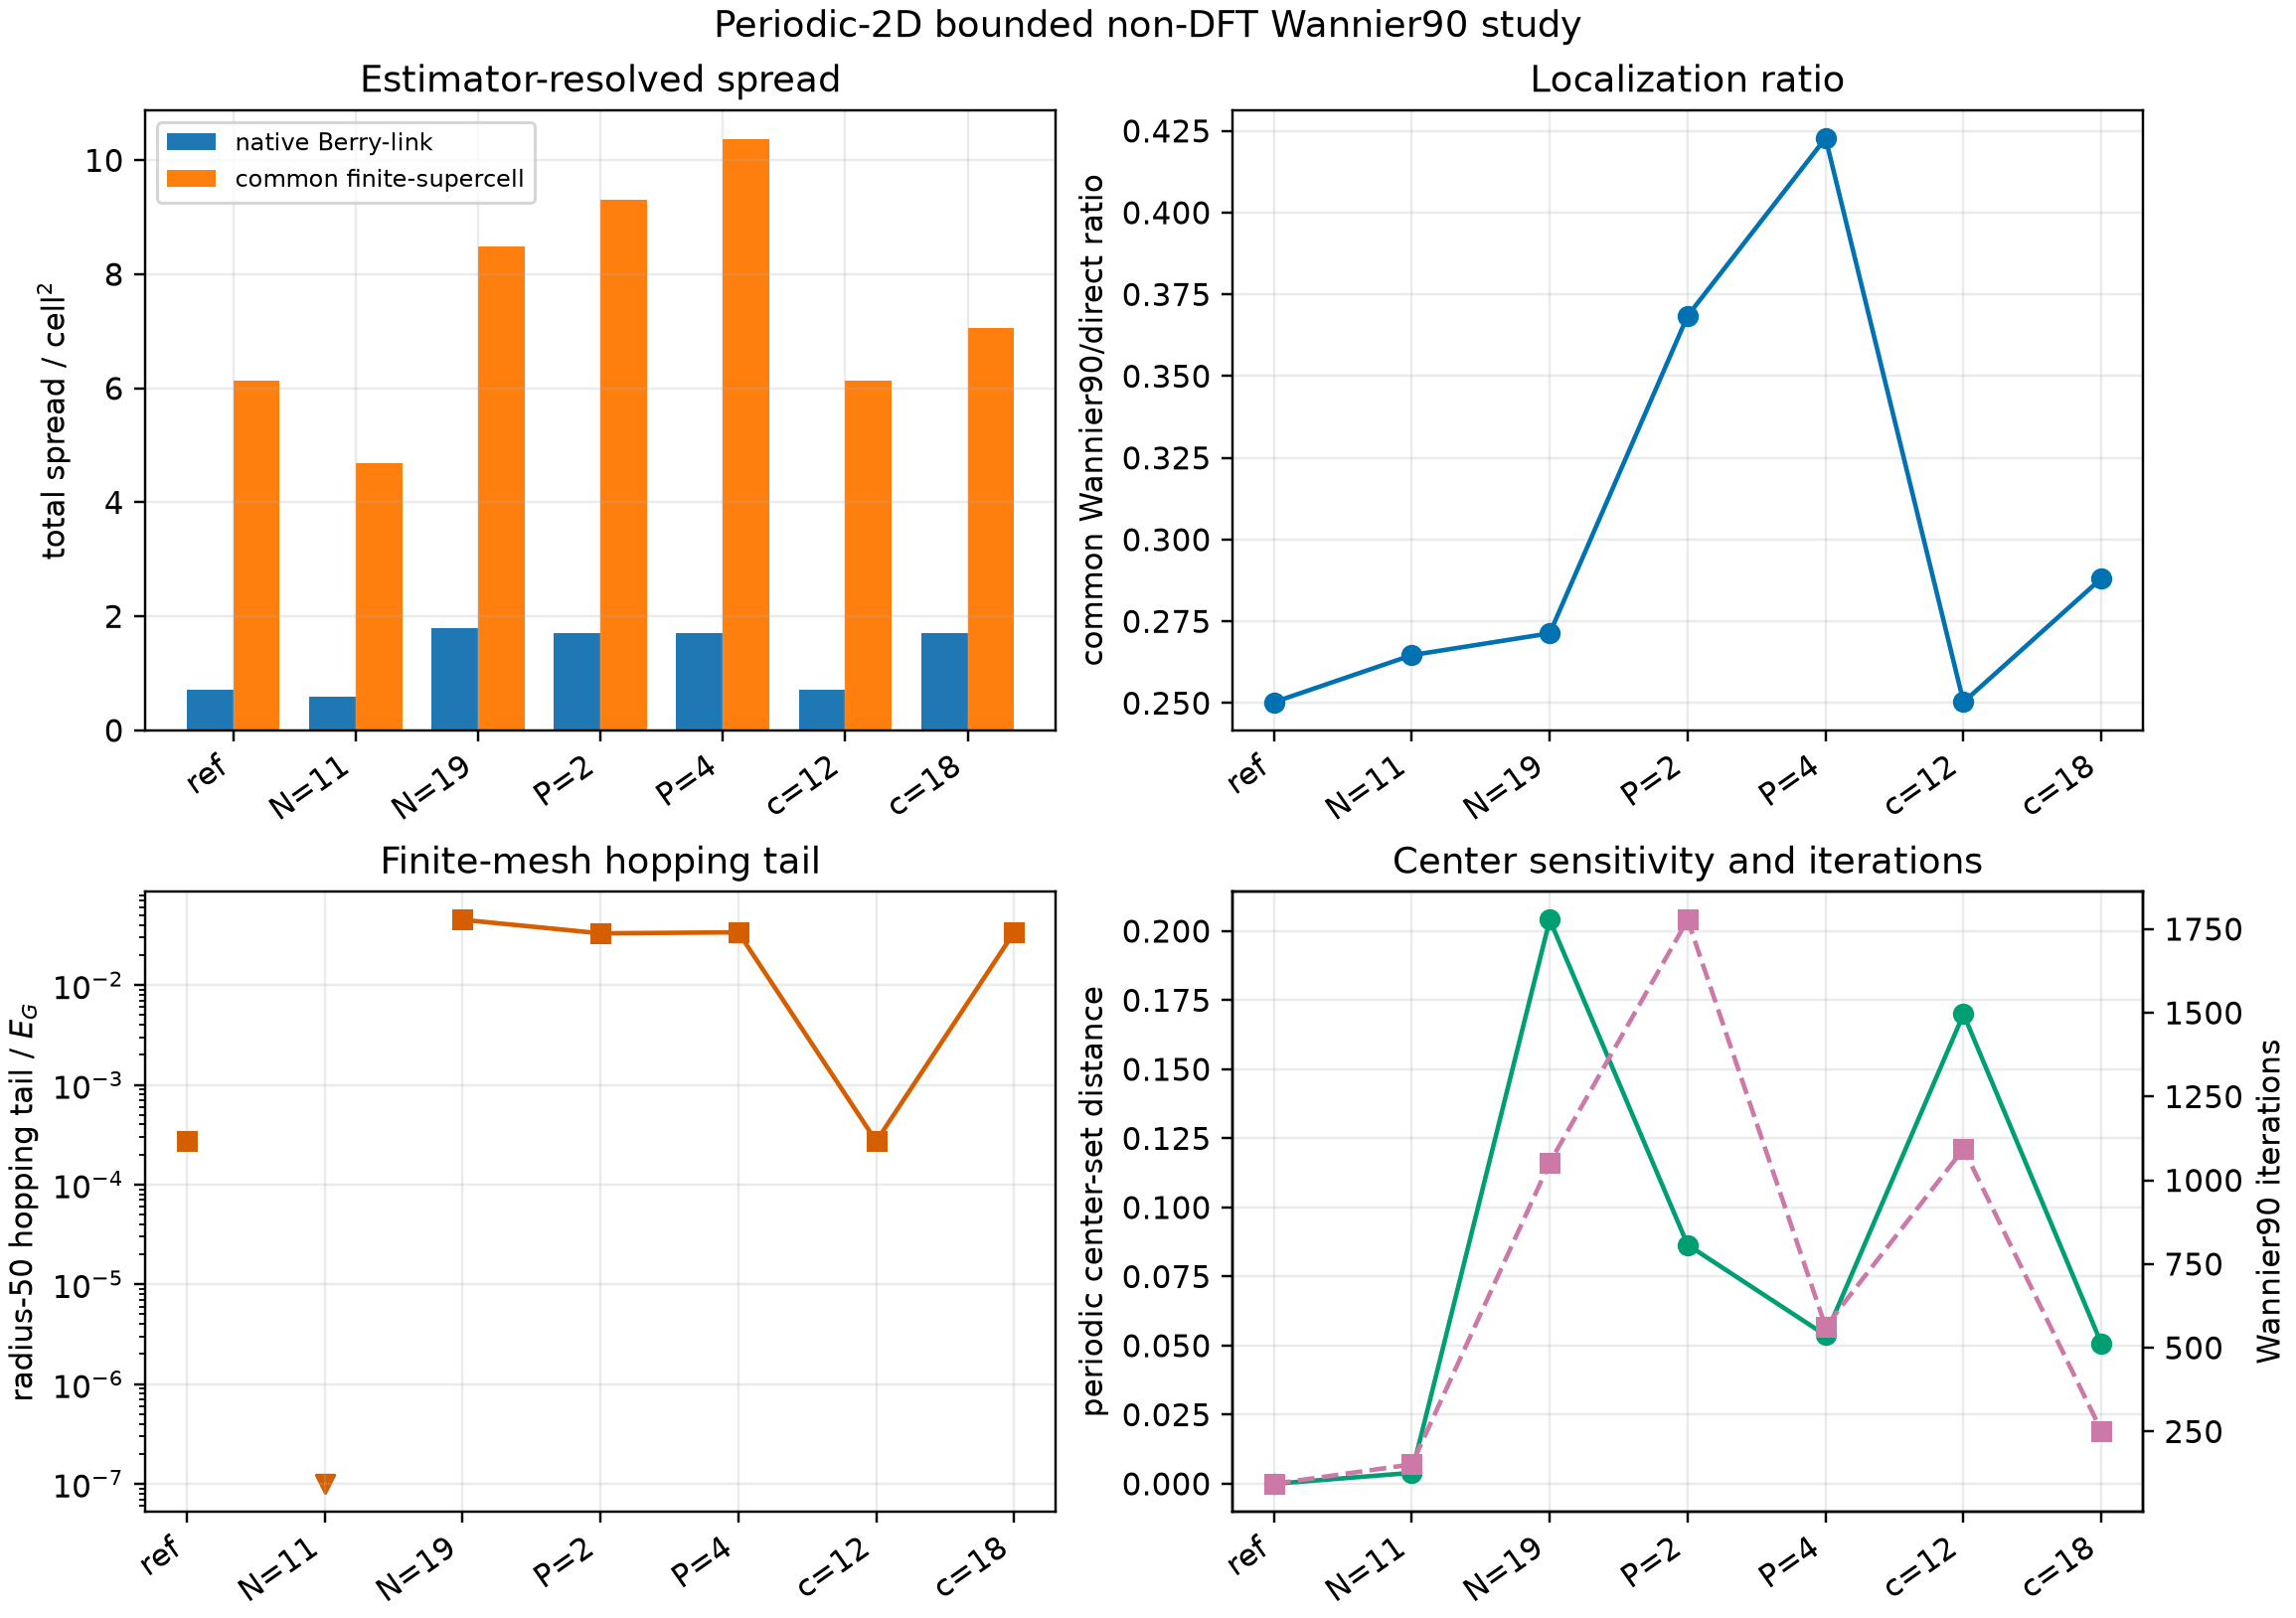
\includegraphics[width=\textwidth]{../../../../../calculations/research-monograph/periodic-2d/wannier90-study-summary.png}
\caption{Extracted Wannier90 sensitivity record. Mesh, plane-wave cutoff, and inactive
embedding variations reach nonmonotone spreads, tails, centers, and optimizer iteration
counts. The zero radius-50 tail for $N=11$ is finite-support bookkeeping, not an
infinite-range conclusion.}
\label{fig:wannier90-sensitivity}
\end{figure}

No predecessor threshold~\cite{Ragasa2026a}, finite-angle inventory, mesh, tolerance,
source identity, or evidence identity is transferred into the higher-rank experiment. A
new calculation requires its own protocol, schemas, verifier, convergence result, and
evidence qualification.
